\begin{figure*}[t!]
\centering
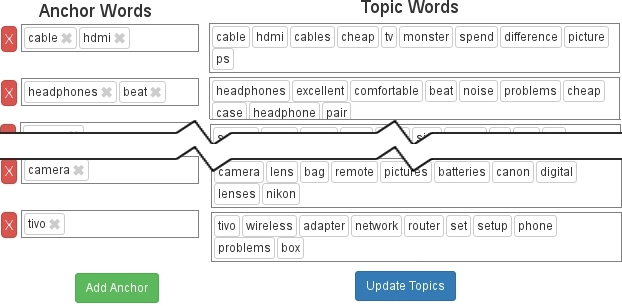
\includegraphics[width=.6\linewidth]{\filename{figures/tbuie}}
\caption{Interface for user study with multiword anchors applied to
interactive topic modeling.}
\label{fig:tbuie}
\end{figure*}

\section{Interactive Anchor Words}
\label{sec:interactive-experiments}

Given high quality anchor facets, the tandem anchor
algorithm can produce high quality topic models (particularly when the
harmonic mean combiner is used).
Moreover, the tandem anchor algorithm is fast enough to be interactive (as
opposed to model-based approaches such as the Interactive Topic Model).
We now turn our attention to our main experiment:
tandem anchors applied to the problem of interactive topic modeling.
We compare both single word and tandem anchors in our study.
We do not include the Interactive Topic Model or Utopian, as
their run times are too slow for our users.

\subsection{Interface and User Study}

To show that interactive tandem anchor words are fast, effective, and
intuitive, we ask users to understand a dataset using the anchor word
algorithm.
For this user study, we recruit twenty participants drawn from a university
student body.
The student median age is twenty-two.
Seven are female, and thirteen are male.
None of the students had any prior familiarity with topic
modeling or the \twentynews{} dataset.

Each participant sees a simple user interface
(Figure~\ref{fig:tbuie}) with topic given as a row with two columns.
The left column allows users to view and edit topics' anchor words;
the right column lists the most probable words in each
topic.\footnote{While we use topics generated using harmonic mean for
  our final analysis, users were shown topics generated using
  the min combiner.  However, this does not change our result.}
The user can remove an anchor word or drag words from the topic word lists
(right column) to become an anchor word.
Users can also add additional topics by clicking the ``Add Anchor'' to create
additional anchors.
If the user wants to add a word to a tandem anchor set that does not
appear in the interface, they manually type the word (restricted
to the model's vocabulary).
When the user wants to see the updated topics for their newly refined
anchors, they click ``Update Topics''.

We give each a participant a high level overview of topic modeling.
We also describe common problems with topic models including intruding topic
words, duplicate topics, and ambiguous topics.
Users are instructed to use their best judgement to determine
if topics are useful.
The task is to edit the anchor words to improve
the topics.
We asked that users spend at least twenty minutes, but no more than thirty
minutes.
We repeat the task twice: once with tandem anchors,
and once with single word anchors.\footnote{The order users complete these tasks is counter-balanced.}

\begin{figure*}[t!]
\centering
\includegraphics[height=.9\linewidth,angle=90]{\filename{auto_fig/user_acc}}
\caption{Classification accuracy and coherence using topic features gleaned from
user provided multiword and single word anchors. Grahm-Schmidt anchors are
provided as a baseline. For all metrics except \abr{vi}, higher is better.
Except for coherence, multiword anchors are best.}
\label{fig:user-accuracy}
\end{figure*}

\begin{figure*}[t!]
\centering
\includegraphics[height=.9\linewidth,angle=90]{\filename{auto_fig/significance}}
\caption{Topic significance for both single word and
multiword anchors. In all cases higher is better. Multiword anchors produce
topics which are more significant than single word anchors.}
\label{fig:user-significance}
\end{figure*}


\subsection{Quantitative Results}

We now validate our main result that for interactive topic modeling, tandem
anchors yields better topics than single word anchors.
Like our title-based experiments in Section~\ref{sec:oraclular-experiments},
topics generated from users become features to train and test a classifier for
the \twentynews{} dataset.
We choose this dataset for easier comparison with the Interactive Topic
Modeling result of~\newcite{hu-14:itm}.
Basedsie on our results with title-based anchors, we use the harmonic mean
combiner in our analysis.
As before, we report not only accuracy, but also multiple
clustering metrics using the confusion matrix from the classification task.
Finally, we report topic coherence.

Figure~\ref{fig:user-accuracy} summarizes
the results of our quantitative evaluation.
While we only compare user generated anchors in our
analysis, we include the unsupervised Gram-Schmidt anchors as a baseline.
Some of the data violate assumptions of normality.
Therefore, we use Wilcoxon's signed-rank test~\cite{wilcoxon-test} to determine
if the differences between multiword anchors and single word anchors are
significant.

Topics from user multiword anchors yield higher
classification accuracy (Figure~\ref{fig:user-accuracy}).
Not only is our approach more scalable than the Interactive Topic Model, but we
also achieve higher classification accuracy than~\newcite{hu-14:itm}.\footnote{However, the values are not strictly comparable, as \newcite{hu-14:itm} use
the standard chronological test/train fold, and we use random splits.}
Tandem anchors also improve clustering
metrics.\statsiguser{}

While user selected tandem anchors produce better classification features than
single word anchors,
users selected single word anchors produce topics with similar topic
coherence scores.\footnote{The difference between coherence
scores was \emph{not} statistically significant using Wilcoxon's signed-rank
test.}


To understand this phenomenon, we use quality metrics~\cite{junk-topic} for
ranking topics by their correspondence to genuine themes in the data.
Significant topics are likely skewed toward a few related words, so
we measure the distance of each topic-word distribution from the {\bf uniform}
distribution over words.
Topics which are close to the underlying word distribution of the entire data
are likely to be {\bf vacuous}, so we also measure the distance of each topic-word
distribution from the underlying word distribution.
Finally, {\bf background} topics are likely to appear in a wide range of documents,
while meaningful topics will appear in a smaller subset of the data.

Figure~\ref{fig:user-significance} reports our topic significance findings.
For all three significance metrics, multiword anchors produce more significant
topics than single word anchors.\statsiguser{}
~Topic coherence is based solely on the top $n$ words of a topic, while both
accuracy and topic significance depend on the entire topic-word distributions.
With single word anchors, topics with good coherence may still be too general.
Tandem anchors enables users to produce topics with more specific word distributions which
are better features for classification.

\begin{table*}[t!]
\begin{center}
\small
\begin{tabular}{p{.20\textwidth} p{.45\textwidth}}
\hline\hline
\bf Anchor & \bf Top Words in Topic\\\hline
\hline\multicolumn{2}{l}{\bf Automatic Gram Schmidt}\\\hline
\rowcolor{gray!35} love & love god evolution romans heard car \\
game & game games team hockey baseball heard \\
\hline\multicolumn{2}{l}{\bf Interactive Single-word}\\\hline
\rowcolor{gray!35}evolution & evolution theory science faith quote facts \\
religion & religion god government state jesus israel \\
\rowcolor{gray!35}baseball & baseball games players word teams car \\
hockey & hockey team play games season players \\
\hline\multicolumn{2}{l}{\bf Interactive Tandem}\\\hline
\rowcolor{gray!35}atheism god exists prove & god science evidence reason faith objective \\
christian jesus & jesus christian christ church bible christians \\
\rowcolor{gray!35}jew israel & israel jews jewish israeli state religion \\
baseball bat ball & hit baseball ball player games call \\
\rowcolor{gray!35}hockey nhl & team hockey player nhl win play \\
\end{tabular}
\end{center}
\caption{Comparison of topics generated for \twentynews{} using various types
of anchor words. Users combine words to create more specific
topics with tandem anchors.}
\label{tab:qual}
\end{table*}


\subsection{Qualitative Results}

We examine the qualitative differences between how users
select multiword anchor facets versus single word anchors.
Table~\ref{tab:qual} gives examples of topics generated using different
anchor strategies.
In a follow-up survey with our users, 75\% find
it easier to affect individual changes in the topics using tandem anchors
compared to single word anchors.
Users who prefer editing multiword anchors over single word anchors
often report that multiword anchors make it easier to merge similar
topics into a single focused topic by combining anchors.
For example, by combining words related to \underline{Christianity}, users create
a topic which is highly specific, and differentiated from general
religion themes which also include Atheism and Judaism.

While users find that use tandem anchors is easier, only 55\% of our users
say that they prefer the final topics produced by tandem anchors compared
to single word anchors.
This is in harmony with our quantitative measurements of topic coherence, and
may be the result of our stopping criteria: when users judged the topics to be
useful.

However, 100\% of our users feel that the topics created through interaction
were better than those generated from Gram-Schmidt anchors.
This was true regardless of whether we used tandem anchors or single word
anchors.

Our participants also produce fewer topics with multiword anchors.
The mean difference between topics under single word anchors and
multiple word anchors is $9.35$.
Follow up interviews reveal that participants resolve ambiguous topics
by creating a new anchor
for each of the ambiguous terms, thus explaining the proliferation of topics
for single word anchors.
In contrast, fixing an ambiguous tandem anchor is simple: users just add more
terms to the anchor facet.
